%!TEX root = ../book.tex
\chapter{Sensors}\label{chap:sensors}
Robots are systems that sense, actuate, and compute. So far, we have studied the basic physical principles of motion, i.e., locomotion and manipulation. We now need to understand the basic principles of robotic sensors that provide the necessary data for a robot to make decisions and control its body.
%
The goals of this chapter are:
\begin{itemize}
\item provide an overview of sensors commonly used on robotic systems,
\item outline the physical principles behind the functioning of sensors,
\item clarify the mechanisms responsible for uncertainty in sensor-based reasoning.
\end{itemize}

% \section{Robotic Sensors}
Historically, the development of robotic sensors is driven by industries other than robotics. These include submarines, automatically opening doors, safety devices for industry, servos for remote-controlled toys, and more recently cellphones, automobiles and gaming consoles. These industries are mostly responsible for making ``exotic'' sensors available at low cost by identifying mass-market applications.
For example, accelerometers and gyroscopes are now widely used in smartphones and cost less than a dollar; the XBox gaming console made 3D depth sensing (through the Kinect) accessible for a greatly lower cost than before.

\begin{mdframed}
Think about the sensors that you are interacting with daily. What sensors do you have in your phone, in your kitchen, or in your car?
\end{mdframed}

As we will see later on, sensors are hard to classify by their application domain and target use case. In fact, most problems benefit from every possible source of information they can obtain. For example, localization can be achieved by measuring how many degrees a wheel has turned with a sensor known as ``encoder'' (cf. \cref{sec:sensors:encoders}); however, estimation becomes more precise with the addition of accelerometers (\cref{sec:sensors:inertia}) or even vision sensors (\cref{chap:vision}). All of these approaches differ drastically in their precision and the kind of data they provide, but none of them is able to completely solve the localization problem on its own.
Consequently, this chapter is organized according to the physical quantities a sensor is measuring, rather than the higher-level estimates it can contribute to measure.

\begin{mdframed}
Think about the kind of data that you can obtain from an encoder, an accelerometer, or a vision sensor on a non-holonomic robot. What are the fundamental differences? What physical principles do they leverage?
\end{mdframed}

Although an encoder is able to measure position, it is used in this function only on robotic arms. If the robot is non-holonomic, closed paths in its configuration space (i.e., robot motions that return the encoder values to their initial position), do not necessarily drive the robot back to its starting point (as exemplified in \cref{fig:holonomy}).
In those robots, encoders are therefore mainly utilized to measure speed. An accelerometer instead, by definition, measures the derivative of speed. Vision, finally, allows to calculate the absolute position (or the integral of speed) if the environment is equipped with unique features. An additional fundamental difference between those three sensors is the amount and kind of data they provide. An accelerometer samples real-valued quantities that are digitized with some precision. An odometer instead delivers discrete values that correspond to encoder increments. Finally, a vision sensor delivers an array of digitized real-valued quantities (namely colors). Although the information content of this sensor exceeds that of the other sensors by far, cherry-picking the information that is really useful to complete the task remains a hard, and largely unsolved, problem.


\section{Terminology}\label{sec:sensors:terminology}

When dealing with sensors, it is important to provide precise definitions of terms such as ``speed'' and ``resolution'', as well as additional taxonomy that is specific to robotics.
%
Roboticists differentiate between \textsl{active} and \textsl{passive} sensors. Active sensors \index{Active sensor} emit energy of some sort and measure the reaction of the environment. Passive sensors \index{Passive sensor} instead measure energy from the environment. For example, most distance sensors (\cref{sec:sensors:light}) are active sensors, because they sense the reflection of a signal they emit; conversely, an accelerometer, a compass, or a push-button are passive sensors.

Another important term to characterize sensors is its \textsl{range}\index{Range (sensor)}, i.e. the \textsl{difference} between the upper and the lower limit of the quantity a sensor can measure.
This differs from its \textsl{dynamic range}\index{Dynamic Range (sensor)}, which is the \textsl{ratio} between the highest and lowest value a sensor can measure. It is usually expressed on a logarithmic scale (to the basis 10), also known as ``decibel''\index{Decibel}. The minimal distance between two values a sensor can measure is known as its \index{Resolution (sensor)} \textsl{resolution}. The resolution of a sensor is primarily limited by the physical principle it leverages (e.g., a light detector can only count multiples of a quant), however it is usually limited by the analog-digital conversion process.
The resolution of a sensor should not be confused with its accuracy or its precision (which are two different concepts). For example, even though an infrared distance sensor might produce $4096$ different values to encode distances from $0$ to $10cm$ (which suggests a resolution of around $24$ micrometers), its precision is much lower than its resolution (usually in the order of millimeters) due to noise in the acquisition process.

A sensor's \textsl{accuracy}\index{Accuracy (sensor)} is the difference between its (average) output $m$ and the true value $v$ to be measured:
\begin{equation}
accuracy=1-\frac{|m-v|}{v}
\end{equation}
This measure provides a quantity that approaches $1$ for very accurate values and $0$ if the measurements group far away from the actual value. In practice, however, this measure is rarely used and accuracy is provided with absolute values or a percentage at which a value might exceed the true measurement.

A sensor's \textsl{precision}\index{Precision (sensor)} instead is given by the ratio of range and statistical variance of the signal.
As detailed in \cref{fig:precision}, precision is therefore a measure of \textsl{repeatability} of a signal, whereas accuracy describes a \textsl{systematic error} that is introduced by the sensor's physics.
\begin{figure}
	\centering
	% 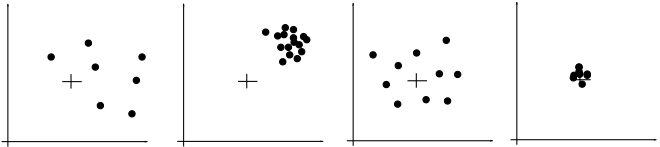
\includegraphics[width=0.9\textwidth]{figs/precisionvsaccuracy.png}
	\def\svgwidth{0.9\textwidth}
    \import{./figs/}{precisionvsaccuracy.pdf_tex}
	\caption{The cross corresponds to the true value of the signal. From left to right: neither precise nor accurate, precise but not accurate, accurate but not precise, accurate and precise.
	\label{fig:precision}}
\end{figure}
%
For example, a GPS sensor is usually precise within a few meters, but only accurate to tens of meters. This becomes most obvious when satellite configurations change, resulting in the precise region jumping by a couple of meters. In practice, this can be avoided by fusing this data with other sensors, e.g.\ from an IMU.

The speed at which a sensor can provide measurements is known as its \index{Bandwidth (sensor)} \textsl{bandwidth}. For example, if a sensor has a bandwidth of 10 Hz, it will provide a signal ten times a second. This is important to know, as querying the sensor more often is a waste of computational time and potentially misleading.


\section{Proprioception vs. Exteroception}
\label{sec:sensors:proprioception}

Anotehr important taxonomy is the difference between proprioception and exteroception.
\textsl{Proprioception}\index{Proprioception} refers to the perception of the internal state of a robot.
Proprioception includes estimation of the robot's joint angles, its speeds, as well as internal torques and forces.
%
% Finally, there are other means of proprioception, such as simple sensors that can detect when a robot gets picked up, e.g.
%
%\section{Exteroception of the physical interaction with the environment}
\label{sec:sensors:interaction}
%
Conversely, \textsl{exteroception}\index{Exteroception} refers to sensing anything outside of the physical embodiment the robot. Exteroception is important because it is crucial for the robot to correctly perceive the state of the world, estimate the uncertainties related to it, and properly act based upon these uncertainties.
Importantly, while the majority of sensor development focuses on \textsl{distal} sensors capable of measuring quantities in the far space (e.g. cameras, see \cref{chap:vision}, or sound-based sensors, see \cref{sec:sensors:sound}), in recent years more attention has been given to \textsl{proximal} sensors, that are concerned with measuring the environment that is immediately surrounding the body or even directly on the robot body.
Applications of this technology are varied, from tasks that require measuring and controlling the interaction of the end-effector with the environment (e.g. sanding a table with a fixed vertical force), to manipulating in clutter---where contact with obstacles is inevitable.

\begin{mdframed}
In robotics, it often helps to make comparisons with human performance.
How many daily tasks \textsl{do not} require physical interaction with the environment?
If they do, would you be able to successfully complete them without contact, and how would your performance decrease if you were to ``avoid collisions at all costs''?
\end{mdframed}

%\section{Proprioception of the internal state of the robot}\label{sec:sensors:proprioception}

\section{Sensors that measure the robot's joint configuration}\label{sec:sensors:encoders}

The most important proprioceptive sensor is the \textsl{encoder}\index{Encoder}. Encoders can be used for sensing joint position and speed, as well as force---if used in conjunction with a spring. Encoders can be divided in incremental (relative, used primarily in mobile robotics) and absolute encoders (mainly used in robot manipulators).
%The latter are mostly used in industrial applications, but are not common in mobile robotics.
In general, they rely on either a magnetic or optical beacon turning together with the motor and being sensed by an appropriate sensor that counts every pass-through. The most common encoder in robotics is the \textsl{quadrature encoder}\index{Quadrature encoder}, which is an optical encoder. It relies on a pattern rotating with the motor and an optical sensor that can register black/white transitions, as shown in Figure~\ref{fig:encoders}.

\begin{figure}
	\centering
		\includegraphics[width=0.3\textwidth]{figs/encoderdisk.png}
		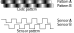
\includegraphics[width=0.3\textwidth]{figs/quadraturencoder.png}
		\includegraphics[width=0.3\textwidth]{figs/absoluteencoder.png}
	\caption{From left to right: encoder pattern used in a quadrature encoder, resulting sensor signal (forward motion), absolute encoder pattern (gray coding).}
	\label{fig:encoders}
\end{figure}

While a single sensor would be sufficient to detect rotational position and speed, it does not allow to determine the direction of motion. Quadrature encoders therefore have two sensors, A and B, that register an interleaving pattern with distance of a quarter phase. If A leads B, the disk is rotating in a clockwise direction. If B leads A, then the disk is rotating in a counter-clockwise direction. It is also possible to create absolute encoders---an example of which is shown in Figure~\ref{fig:encoders}, right. This pattern is a 3-bit pattern that encodes 8 different segments on a disc. Notice that the pattern is arranged in such a way that there is only one bit changing from one segment to the other. This is known as ``Gray code''\index{Gray code}.
% The function of linear encoders is analogous, both for incremental and absolute encoders.

If combined with a spring, such as in a \textsl{Series Elastic Actuator}\index{Series Elastic Actuator}, rotary and linear encoders can be used as simple force or torque sensors using Hooke's law ($F=kx$, where $k$ is a spring constant).
This can be used when operating a robot under a static (\cref{sec:forces:statics}) or dynamic level of abstraction.
% Whereas the series elastic actuator is the most illustrative examples, most load cells operate on the premise of measuring displacements within materials of known properties. Here, measuring changes in resistance or capacitance might be easier choices.
Another method to estimate the actual force or torque acting on a joint is to measure the current consumed at each joint. Knowing a mechanism's pose allows to calculate the resulting forces and torques across the mechanism as well as the currents required for empty loading conditions. Derivations of these then correspond to additional forces that can hence be calculated.

\section{Measuring force}

The measurement of physical interaction forces is of paramount importance for robotics.
It enables a variety of capabilities that humans take from granted, from gently picking a strawberry to safely engaging in touch-based interactions with humans.
While the development of robust, scalable, and miniaturizable force sensors is still matter of active research, the most widespread device to date is the \textsl{Force/Torque (or F/T) sensor}\index{Force/Torque sensor}. It is a mechanical device that is capable of detecting one or more components of a six-dimensional wrench applied to it (i.e. a 3D force and a 3D torque, see \cref{sec:forces:statics}).
To date, most commercially available F/T sensors use \textsl{strain gauges}---and in particular, at least one strain gauge per axis of detection. Simply put, a strain gauge is a metal (i.e. conductive) foil that changes its shape when a wrench is applied to it, and while doing so it changes its electrical resistance (which can then be measured with appropriate circuitry).
While precise, F/T sensors are plagued by a number of limitations: 1) high costs; 2) size (a standard F/T sensor is usually the size of a human wrist); 3) low signal-to-noise ratio; 4) low bandwidth/responsivity; 5) a single data point that is sparse in space and time.

\section{Measuring pressure or touch}

In order to partially mitigate the above issues with force sensing, roboticists have worked on a complementary capability, that is measuring the pressure applied on the robot's surface.
A pressure sensor is a device that is capable of detecting either a contact/collision as a binary data (in which case is generally referred to as touch sensor), or a gradient of pressure applied to it.
In general, the vertical pressure applied to the sensor is proportional to the 1D vertical force that is applied to the direction normal to the sensor, and this makes a pressure sensor a good substitute to F/T sensors in specific applications (e.g. grasping).
Additionally, pressure sensors are mostly based on measuring pressure through a change in \textsl{capacitance} rather than resistance (no different from the functioning of a touchscreen on a modern smartphone): when pressure is applied to a capacitor-like device (i.e. two conductive plates separated by an insulating material), the distance between the two plates reduces and this causes a change in capacitance which can be readily measured.
If compared to F/T sensors, pressure sensors provide limited amount of information ($1$-dimensional vs $6$-dimensional), but they allow for: 1) high responsiveness; 2) high density of sensing (up to tens of sensors per $cm^2$); 3) low cost; 4) ease of miniaturization.

\section{Artificial skins for robotics}

The human sense of touch is the oldest, the largest, and the most important of our senses.
To humans, contact and physical interaction are a resource rather than an impediment, and we are surprisingly proficient at leveraging touch in a variety of situations.
Therefore, it is natural for roboticists to equip robots with similar capabilities in order to achieve performance levels comparable to humans'.
To date, there are no commercially available whole-body artificial skins for robots; however, a number of efforts (from both established robot manufacturers and startups) are showing promising prototypes.
Interestingly, researchers are taking full advantage of the recent developments in a variety of different technologies, and are creating dense arrays of artificial sensors that combine one or more of the following sensing modalities: interaction forces (\cref{sec:sensors:interaction}), sound (\cref{sec:sensors:sound}), light (\cref{sec:sensors:light}), cameras (\cref{chap:vision}), inertia-based sensors (\cref{sec:sensors:inertia}), and more.

\section{Sensors using light}\label{sec:sensors:light}

The small form factor and low price of light-sensitive semi-conductors have led to a proliferation of light-based sensors relying on a multitude of physical effects. These include reflection, phase shift, and time of flight.

\subsection{Reflection}
Reflection is one of the easiest and most immediate principles to take advantage of: the closer an object is, the more it reflects light shined at it. This allows to easily measure distance to objects that reflect light well and that are not too far away. In order to make these sensors as independent from an object's color as possible (but unfortunately not totally independent), infrared is most commonly chosen wavelength.
A reflection-based distance sensor is made from two components: an emitter (that emits an infrared signal) and a receiver (tasked with measuring the strength of the reflected signal). A typical response is shown in Figure~\ref{fig:epuckir}. The values obtained at an analog-digital converter correspond to the voltage at the infrared receiver and are saturated for low distances (flat line), and quadratically decrease afterwards.

\begin{figure}
	\centering
		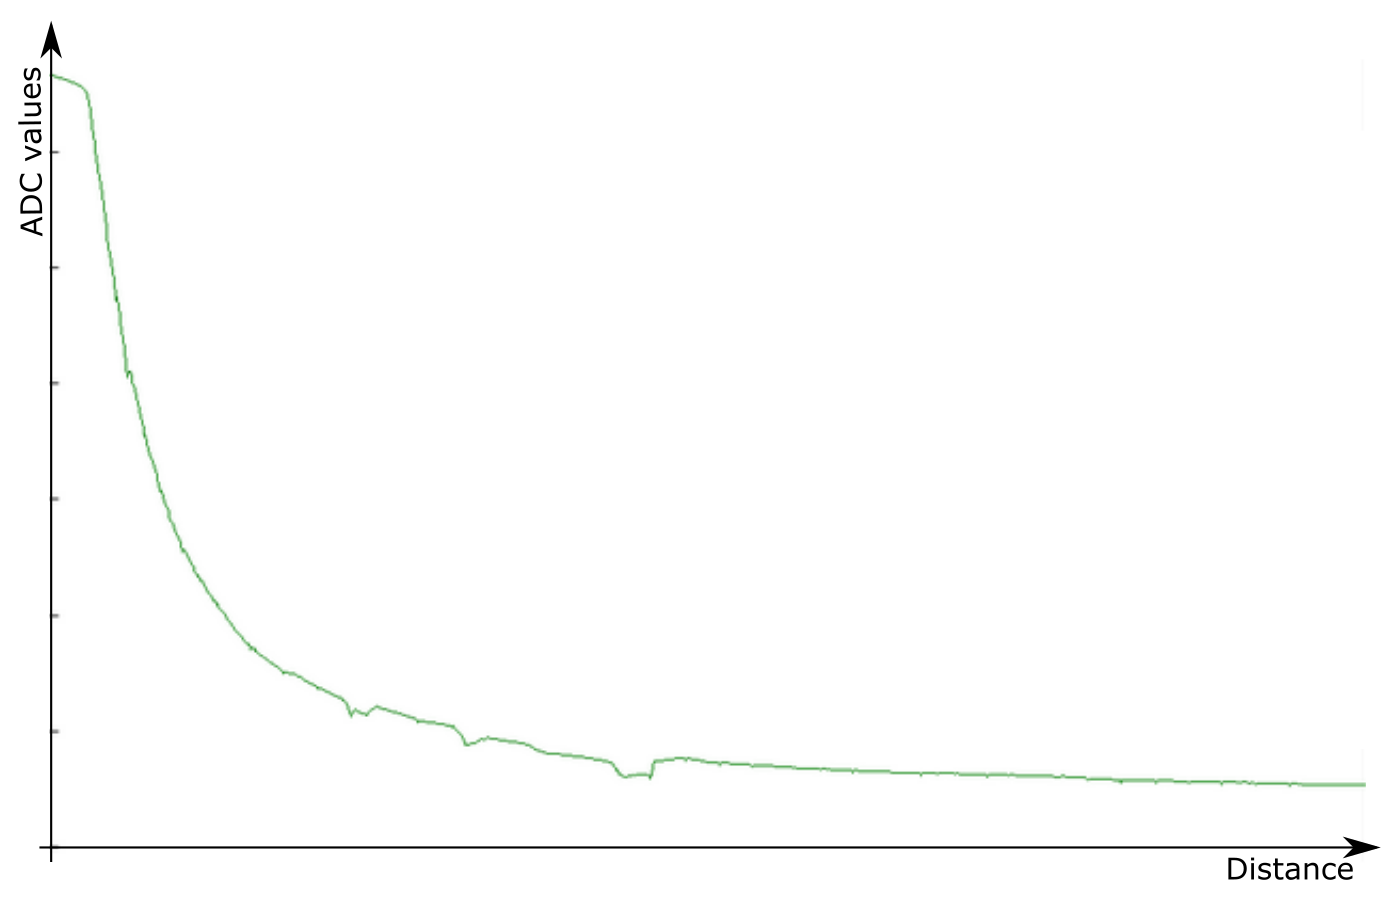
\includegraphics[width=0.8\textwidth]{figs/epuckirsensor.png}
	\caption{Typical response of an infrared distance sensor as a function of distance. Units are left dimensionless intentionally.}
	\label{fig:epuckir}
\end{figure}

Using more than one infrared sensor/emitter pair---e.g., using a projector as emitter and a camera as receiver---not only allows to measure the distance of many points at once, but also to assess the structure of the environment by calculating its impact on the deformation of patterns. For example, a straight line becomes a curve when projected onto a round surface. This approach is known as \textsl{structured light}\index{Structured light} and is illustrated in Figure~\ref{fig:struclight}.
Thanks to the continuously increasing efficiency of computational systems, a light-weight version of such an approach has become feasible to be implemented at small scale and low cost around 2010, and emerged as a novel standard in robotic sensing.

\begin{figure}
	\centering
		\includegraphics[width=\textwidth]{figs/structuredlight.png}
	\caption{From left to right: two complex physical objects, a pattern of colored straight lines and their deformation when hitting the surfaces, reconstructed 3D shape. From \protect\cite{zhang2002rapid}.}
	\label{fig:struclight}
\end{figure}

Instead of using line patterns, infrared-based depth image sensors use a speckle pattern (a collection of randomly distributed dots with varying distances), and two computer vision concepts: \textsl{depth from focus} and \textsl{depth from stereo}.\index{Depth from Focus}\index{Depth from Stereo} When using a lens with a narrow focal depth, objects that are closer or farther away appear blurred (you can easily observe this on professional portrait photos, which often use this effect for aesthetic purposes under the name of ``bokeh'').
Measuring the ``blurriness'' of a scene (for known camera parameters) therefore allows an initial estimate of depth.
Conversely, depth from stereo works by measuring the disparity of the same object appearing in two images taken by cameras that are a known distance apart. Being able to identify the same object in both frames allows to calculate this disparity, and from there the distance of the object: the farther the object is, the smaller the disparity will be.
This is where the speckle pattern comes in handy: it simply requires to search for blobs with similar size that are close to each other.

\subsection{Phase shift}\label{sec:phaseshiftsensors}

As you detailed in Figure~\ref{fig:epuckir}, reflection can only be precise if distances are short. Instead of measuring the strength (aka amplitude) of the reflected signal, laser distance sensors measure the phase difference of the reflected wave. In order to do this, the emitted light is modulated with a wave-length that exceeds the maximum distance the scanner can measure.
If you were to use visible light and to do so at much slower speeds, you would see a light that keeps getting brighter, then getting darker, briefly turns off and then starts getting brighter again.
Thus, if you were to plot the amplitude of the emitted signal over time (i.e., its brightness), you would see a wave that crosses zero when the light is dark.
As light travels, this wave propagates through space with a constant distance (the wavelength) between its zero crossings. When it gets reflected, the same wave travels back (or at least parts of it that get scattered right back). For example, modern laser scanners\index{Laser range finder} emit signals with a frequency of 5 MHz (turning off 5 million times in one second). Together with the speed of light of approximately $300,000km/s$, this leads to a wavelength of $60m$ and makes such a laser scanner useful up to $30m$.

When the laser is now at a distance that corresponds exactly to one half the wave-length, the reflected signal it measures will be dark at the exact same time its emitted wave goes through a zero-crossing. Going closer to the obstacle results in an offset that can be measured. As the emitter knows the shape of the wave it emitted, it can calculate the phase difference between emitted and received signal. Knowing the wave-length it can now calculate the distance. As this process is mostly independent from ambient light, the estimates can be very precise.
% This is in contrast to a sensor that uses signal strength. As the signal strength decays at least quadratically, small errors, e.g.\ due to fluctuations in the power supply that drives the emitting light, noise in the analog-digital converter, or simply differences in the reflecting surface have drastic impact on the accuracy and precision (see below for a more formal definition of this term).

As the laser distance measurement process is fast, such lasers can be combined with rotating mirrors to sweep larger areas, known as \textsl{Laser Range Scanners}\index{Laser Range Scanners} or \textsl{Lidars}\index{Lidar}. Such systems have been combined into packages consisting of up to $64$ scanning lasers and are nowadays vastly used in the autonomous driving space as they are capable of providing a depth map around a car while driving.
It is also possible to modulate projected images with a phase-changing signal, which is the operational principle of early ``time-of-flight'' cameras, which however is not an accurate description of their operation.

\subsection{Time-of-flight}

The most precise distance measurements light can provide is by measuring its time of flight. This can be done by counting the time a signal from an emitter becomes visible in a receiver. As light travels very fast ($3\cdot10^8m/s$), this requires high-speed electronics that can measure time periods smaller than nanoseconds in order to achieve centimeter accuracy.
In practice, this is done by combining the receiver with a very fast electronic shutter that operates at the same frequency of the emitted light. As this timing is known, one can infer the time light has traveled by measuring the quantity of photons that made it back from the reflective surface within one shutter period.
As an example, light travels $15m$ in $50ns$. Therefore, it will take a pulse of $50ns$ to return from an object at a distance of $7.5m$. If the emitter transmits a pulse of $50ns$ length and then closes the receiver with a shutter, the receiver will receive more photons the closer the object is, but no photons if the object is farther than $7.5m$. Given a fast enough and precise circuit that acts as a shutter, it is sufficient to measure the actual amount of light that returns from the emitter.

\section{Sensors using sound}\label{sec:sensors:sound}

\subsection{Ultra-sound distance sensors}

An ultra-sound distance sensor operates by emitting an ultra-sound pulse and measures its reflection. Unlike a light-based sensor that measures the amplitude of the reflected signal, a sound-based sensor measures the time it took for the pulse to travel back and forth.
This is possible because sound travels at much lower speed ($3\cdot10^2m/s$) than light ($3\cdot10^8m/s$). The fact that the sensor actually has to wait for the signal to return leads to a trade-off between range and bandwidth (see \cref{sec:sensors:terminology}: allowing a longer range requires waiting longer for the signal to come back, which in turn limits how often the sensor can provide a measurement.
% (Look these definitions up above before you read on.)\td{fix--up above where?}
Although ultrasound distance sensors have become progressively less common in robotics, they have an advantage over light-based sensors: instead of sending out a ray, the ultra-sound pulse results in a cone with an opening angle of $20$ to $40$ degrees. Because of this, such sensors are able to detect small obstacles without the requirement of directly hitting them with a ray. This property makes them the sensor of choice in specific applications, such as the automated parking assist technologies in modern cars.

\subsection{Texture recognition}

Audible sound consists of high frequency vibrations in the range between $20Hz$ and roughly $15kHz$. Microphones are therefore designed to measure vibrations in this range. This allows them to double as the Pacinian corpuscle in human skin cells, which is known to have a resonance frequency of $250Hz$ and is mostly responsible for texture recognition. Indeed, rubbing a texture against a microphone can be used to differentiate between tens and hundreds of different textures \cite{hughes14}. These sensors usually calculate the frequency spectrum of the recorded signal, which can then be classified using machine learning techniques. Being able to recognize a texture by touch is important in applications like grasping and navigation through cluttered terrain.

\section{Inertia-based sensors}\label{sec:sensors:inertia}

A moving mass does not lose its kinetic energy---if there is no friction. Likewise, a resting mass will resist acceleration. Both effects are due to ``inertia'' \index{Inertia} and can be exploited to measure acceleration and speed.

\subsection{Accelerometers}

An accelerometer\index{Accelerometer} can be thought of as a mass on a dampened spring. Considering a vertical spring with a mass attached to it, we can measure the acting force $F=kx$ (Hooke's law\index{Hooke's law}) by measuring the displacement $x$ that the mass has exerted on the spring.
Using the relationship $F=ma$, we can now calculate the acceleration $a$ on the mass $m$. On earth, this acceleration is roughly $9.81\frac{m}{s^2}$.
In practice, these spring/mass systems are realized using microelectromechanical devices (MEMS), such as a cantilevered beam whose displacement can be measured using a capacitive sensor. Accelerometers measure up to three axes of translational accelerations. Inferring an absolute position from it requires a double integration, which introduces significant noise in the estimation and makes position estimates using accelerometers infeasible in practice.
However, as gravity provides a constant acceleration vector, accelerometers are very good at estimating the pose of an object with respect to gravity.

\subsection{Gyroscopes}\label{sec:gyroscopes}

A gyroscope is an electro-mechanical device that can measure rotational orientation. It is complementary to the accelerometer that measures translational acceleration. Classically, a gyroscope consists of a rotating disc that can freely rotate in a system of pivots and gimbals. When moving the system, the inertial momentum maintains the original orientation of the disc, allowing to measure the orientation of the system relative to where the system was originally. A variation of the gyroscope is the rate gyro, which measures rotational/angular velocities.

A rate gyro \index{Rate gyro}\index{Gyroscope} can intuitively be illustrated by considering its \textsl{optical} implementation.
In an optical gyro, a laser beam is split in two and sent around a circular path in two opposite directions. If the device is rotated against the direction of one of these laser beams, one laser will have to travel slightly longer than the other, leading to a measurable phase shift at the receiver.
This phase shift is proportional to the \textsl{rotational speed} of the setup. As light with the same frequency and phase will add to each other and lights with the same frequency but opposite phases will cancel each other, light at the detector will be darker for high rotational velocities.
Importantly, small-scale optical rate gyros are not practical, but MEMS rate gyros are widely available and use a different technology, as they rely on a mass suspended by springs. The mass is actively vibrating, making it subject to Coriolis forces when the sensor is rotated. Coriolis forces can be best understood by moving orthogonally to the direction of rotation on a vinyl disk player. In order to move in a straight line, you will not only need to move forwards, but also sideways. The necessary acceleration to change the speed of this sideways motion is counteracting the Coriolis force, which is both proportional to the lateral speed (the vibration of the mass in a MEMS sensor) and the rotational velocity, which the device wishes to measure. Note that the MEMS gyro would only be able to measure acceleration if it were not vibrating.

Gyroscopes can measure the rotational speed around three axes, which can be integrated to obtain absolute orientation. As an accelerometer measures along three axes of translation, the combination of both sensors can provide information on motion in all six degrees of freedom. Together with a magnetometer (compass), which provides absolute orientation, this combination is also known as \textsl{Inertial Measurement Unit}\index{Inertial Measurement Unit} (or IMU\index{IMU}).

\section{Beacon-based sensors}

Localizing an object by triangulation goes back to ancient civilizations, where sailors oriented themselves using the stars. As stars are only visible during unclouded nights, seafarers have invented systems of artificial beacons emitting light, sound, and eventually radio waves. The most sophisticated of such systems is the Global Positioning System (GPS). GPS consists of a number of satellites in orbit that are equipped with knowledge about their precise location and have synchronized clocks. These satellites broadcast a radio signal that travels at the speed of light and is coded with its time of emission. GPS receivers can therefore calculate the distance to each satellite by comparing time of emission and time of arrival. As not only the position (x,y,z), but also the time difference between the GPS receiver's clock and the synchronized clocks of the satellites is unknown, four satellites are needed to obtain a ``fix''. Due to the way information from the satellites is coded, getting an initial fix can take in the order of minutes, but afterwards it becomes available multiple times per second. GPS measurements are neither precise nor accurate enough for robotics applications, and require to be combined with other sensors, such as IMUs and compasses. Please note that the bearing shown on some GPS receivers you may have access to is calculated from subsequent positions and is therefore meaningless if the robot is not moving.

There exist also a variety of indoor GPS solutions, which consists of either active or passive beacons that are mounted in the environment at known locations. Passive beacons, for example infrared reflecting stickers arranged in a certain pattern or 2D barcodes, can be detected using cameras and their pose can be calculated from their known dimensions. Active beacons instead usually emit radio, ultrasound or a combination thereof, which can then be used to estimate the robot's range to this beacon.

\section*{Take-home lessons}
\begin{itemize}
\item Most of a robot's sensors either address the problem of robot localization or localizing and recognizing objects in its vicinity.
\item Each sensor has advantages and drawbacks that are quantified in its range, precision, accuracy, and bandwidth. Therefore, robust solutions to a problem can only be achieved by combining multiple sensors with differing operation principles.
\item Solid-state sensors (i.e.\ without mechanical parts) can be miniaturized and cheaply manufactured in quantity. This has enabled a series of affordable IMUs and 3D depth sensors that will provide the data basis for localization and object recognition on mass-market robotic systems.
\end{itemize}

\section*{Exercises}\small
\begin{enumerate}
\item Given a laser scanner with an angular resolution of 0.01 rad and a maximum range of 5.6 meters, what is the minimum range $d$ a robot needs to have from an object of 1cm width to definitely sense it, i.e., hit it with at least one of its rays? You can approximate the distance between two rays with the arc length.
\item Why does the bandwidth of a Ultra-sound based distance sensor decrease significantly when increasing its dynamic range, but that of a laser range scanner does not for typical operation?
\item You are designing an autonomous electric car to transport goods on campus. As you are worried about cost, you are thinking about whether to use a laser scanner or an ultra-sound sensor for detecting obstacles. As you drive rather slow, you are required to sense up to 15 meters. The laser scanner you are considering can sense up to this range and has a bandwidth of 10Hz. Assume 300m/s for the speed of sound in the following.
\begin{enumerate}
\item Calculate the time it takes until you hear back from the US sensor when detecting an obstacle 15m away. Assume that the robot is not moving at this point.
\item Calculate the time it takes until you hear back from the laser scanner. Hint: you don’t need the speed of light for this, the answer is in the specs above.
\item Assume now that you are moving toward the obstacle. Which sensor will give you a measurement that is closer to your real distance at the time of reading and why?
\end{enumerate}
\item Pick an educational robot platform of your choice and make a list of its sensors.
\item Construct a simple range scanner by mounting an ultra-sound sensor onto a servo motor. Implement a scanning routine that allows you to collect the raw data and display it on the screen. Can you see simple features such as corners and openings?
\item Explore the internet for do-it-yourself robotics shops. What kind of sensors do they offer? What are the interfaces these sensors provide?
\item Pick a physical sensor that you have access to. Can you design an experiment to characterize its precision and accuracy?
\item Your task is to design a sensor that can detect the remaining void in a parcel for an e-commerce application.
\begin{enumerate}
\item What sensors could you think off that would allow you to measure the volume of the content in the box?
\item What additional sensors could you use assuming the box is moving on a conveyor belt.
\item What additional information would you need to know in order to differentiate between box content, the box itself, and the environment around the box? What sensors could you use to get this information?
\item Additional sensors are not within your budget. What kind of measures could you take to reduce the amount of information required?
\end{enumerate}
\item Your task is to design an autonomous cart that can automatically dock with shelves in the environment.
\begin{enumerate}
\item What kind of sensors could you use to locate the shelf in the environment? Assume that the shelf is the only object in a certain target area.
\item What kind of physical measures could you take to simplify detection of the shelf?
\item  What kind of sensors could you use to detect whether the shelf is in a suitable position for docking?
\item What kind of physical measures could you take to simplify the sensing process?
\end{enumerate}
\item You are designing a competitive controller for the ``Ratslife'' game. What kind of information does the environment provide and what kind of sensor would you need to exploit it?
\end{enumerate}\normalsize
